% !TeX program = xetex
% 本报告由 tectonic（XeTeX 引擎）编译：tectonic result/report.tex
% 所有数据均来自仓库内真实产物：configs/、data/production/manifest.json、
% runs/production-48g/history.json、runs/production-48g-old-split/evaluation.json、
% results/inversion-report/summary.json、inversion/results/train_seed*.log、
% README.md 记录的基准，以及 iNETT 姊妹仓库的 metrics_summary.json。
\documentclass[UTF8,a4paper,11pt]{ctexart}
\usepackage{geometry}
\geometry{margin=2.5cm}
\usepackage{amsmath,amssymb}
\usepackage{booktabs}
\usepackage{graphicx}
\usepackage{multirow}
\usepackage{array}
\usepackage{caption}
\usepackage{float}
\usepackage{hyperref}
\hypersetup{colorlinks=true, linkcolor=black, citecolor=blue, urlcolor=blue}
\captionsetup{font=small, labelsep=quad}
\emergencystretch=2em

\title{\textbf{面波频散正演代理与反演实验技术报告}\\
\large ——\texttt{swave-forward} 项目：百万样本数据集、四头神经代理、\\
基于代理的 L-BFGS-B 反演与监督反演基线的实证评估}
\author{\texttt{swave-forward} v0.1.0 项目组}
\date{2026 年 8 月 10 日}

\begin{document}
\maketitle

\begin{abstract}
\noindent 本报告系统总结 \texttt{swave-forward} 项目（纯 Python 瑞利波正演求解器与神经代理）
已完成的全部工作与真实实验结果，覆盖：确定性地质模型生成与百万样本数据集构建、
共享骨干四模态输出神经代理的训练、基于可微代理的 L-BFGS-B 反演实验
（10 万样本全量单起点群体实验与 400 样本 \(\times\) 100 起点的深度多起点实验，
各含无噪声与 1\% 高斯噪声两种观测情景），以及一条独立的监督直接反演基线
（InverseNet）。所有指标均直接取自仓库归档产物，未做任何修饰。

主要结果：（1）正演求解器完成 100 万样本生产数据集，零恢复、零拒绝，数据完整性
由逐分片 SHA-256 清单保证；（2）正演代理在验证集取得 \(1.82\times10^{-4}\) km/s 的
掩码 MAE（300 轮训练末轮即最优）；（3）反演实验呈现显著的\emph{拟合--恢复分离}现象：
全部 20 万行反演 100\% 收敛，代理频散重构 MAE 仅 0.0064 km/s，但 Vs 恢复 MAE 高达
0.305 km/s（平均相对误差 20.8\%），深部层（1.6 km 以下）误差达 0.7 km/s 量级且呈系统性
负偏差；1\% 观测噪声对恢复精度几乎无影响（成对差 \(+5.6\times10^{-4}\) km/s）；
（4）深度多起点实验仅将 Vs MAE 改善至 0.271 km/s，且 P10--P90 经验区间覆盖率仅
49.7\%（名义 80\%），深部层覆盖率趋近于零；（5）独立训练的监督反演网络 InverseNet
在自身划分协议下取得 26.9 m/s 的测试 MAE，比优化反演低约一个数量级。报告对未达预期的
结果给出诚实分析：误差主要来源并非数值不收敛，而是问题的非唯一性、参考模型派生的
逐层搜索边界对深部的系统性约束，以及监督先验的缺失。
\end{abstract}

\tableofcontents
\newpage

\section{引言}
近地表瑞利波频散反演是浅层横波速度结构成像的核心手段。含低速夹层（low-velocity
layer, LVL）的层状半空间中，频散曲线存在密集的``模式接吻''（mode-kissing）根，
对正演求根的稳健性与反演的非唯一性处理都提出了挑战。本项目以 Pan 与 Chen 的
mode-kissing 参考实现\footnote{Lei Pan and Xiaofei Chen, \emph{Efficient Computation
of Dispersion Curves in Low-Velocity-Layered Half-Spaces}（投稿稿，随附
\texttt{bssa-2025003.1.pdf}）；参考代码 \url{https://github.com/pan3rock/mode-kissing}。}
和 Pan 等人的 QEDispInv 反演框架\footnote{Lei Pan, Jiannan Wang and Xiaofei Chen,
\emph{Surface-Wave Dispersion Curve Computation and Inversion}（投稿稿，随附
\texttt{bssa-2025207.1.pdf}）；参考代码 \url{https://github.com/pan3rock/QEDispInv}。}
为算法来源，以纯 Python（NumPy/Numba/SciPy/PyTorch）实现了完整管线：
确定性模型生成 \(\to\) 物理正演 \(\to\) HDF5 数据集 \(\to\) 神经代理训练
\(\to\) 基于代理的反演 \(\to\) 自动报告。两个参考仓库仅提供算法与测试夹具，不作为
运行时依赖。

固定的生产问题定义为：20 个 Vs 值（0.30--2.60 km/s），19 个 0.1 km 有限层加
1.9 km 起算的半空间；频率 0.5--60.0 Hz、步长 0.5 Hz（120 点）；瑞利波 0--3 阶
模式；模型族包括正常（normal）、低速（LVL）、高速（HVL）与高低耦合（coupled）四类。
全文深度单位为 km，速度为 km/s，频率为 Hz。

本文余下结构：第 \ref{sec:method} 节给出方法，第 \ref{sec:data} 节为数据集构建结果，
第 \ref{sec:surrogate} 节为代理训练与精度，第 \ref{sec:inversion} 节为反演实验主结果，
第 \ref{sec:invnet} 节为监督反演基线对比，第 \ref{sec:discussion} 节讨论未达预期的
结果及其影响，第 \ref{sec:conclusion} 节总结。附录 \ref{app:repro} 列出可复现性与
完整性证据。

\section{方法}\label{sec:method}

\subsection{正演求解器}
正演核心（\texttt{src/swave/secular.py}, \texttt{solver.py}）传播未归一化的
瑞利波 Dunkin \(\delta\) 矩阵，用 TOMS 748 在符号变号区间内求根；标量热路径由
Numba JIT 缓存。初始采样沿用参考实现的模态计数估计。为处理模式接吻，实现了两种
恢复策略：\texttt{degraded}（浅化退化模型的根补充完整模型）与 \texttt{quadratic}
（默认；二次极值在同号区间内补采样，可能含成对靠近根）。二次粗扫描在 4 个目标根加
2 个偏置根后停止，与参考算法的有界搜索一致。高阶模式的合法前导缺口保持掩码；
内部缺口或数值失败仅允许一次有界细化，随后触发确定性模型重生成——代码从不以零值
或插值静默填充缺失物理目标。物理参数：\(\epsilon=0.5\)，\texttt{nfine}=2，
二次迭代 3 次，根容差 \(10^{-8}\)，去重容差 \(10^{-7}\)。

求解器正确性由测试夹具（\texttt{tests/test\_reference.py} 及
\texttt{tests/fixtures}）对照参考实现的可溯源输出验证。

\subsection{确定性地质模型生成与数据集格式}
模型生成（\texttt{geology.py}）由 \((\text{全局种子},\text{样本ID},\text{重试计数})\)
完全确定。背景模型表层 Vs 均匀采样，半空间 Vs 不低于表层 \(+0.6\) km/s；
异常置于第 3--12 层，低速异常为背景的 \((1-\text{对比度})\) 倍、连续 2--3 层。
四类模型目标比例：正常 0.25、低速 0.15、高速 0.10、耦合 0.50。Vp 与密度由
Brocher (2005) 经验关系（\texttt{empirical\_method = brocher05}）从 Vs 换算。

数据集（\texttt{configs/dataset.toml}）：100 万接受样本，100 个分片
（每片 10{,}000），全局种子 20260727，最大重试 8 次。每个
\texttt{shard-NNNNN.h5} 含样本 ID、模型族、20 层 Vs/Vp/密度、
\((4\times120)\) 相速度目标（缺失单元为 NaN）、有效掩码、质量标志与重试计数；
gzip 压缩、临时路径写入、完整关闭后原子重命名。\texttt{manifest.json} 记录配置哈希、
包版本、逐分片 SHA-256、各族接受/拒绝计数与恢复计数；恢复训练或评估前逐分片重新
校验全部数据形状、dtype、样本 ID 摘要、物性不变量、曲线掩码与文件校验和。

\subsection{数据划分策略}
划分仅由 \(\text{样本ID} \bmod 100\) 决定，跨分片稳定：0--79 训练（80\%），
80--84 验证（5\%），85--89 测试（5\%），90--99 反演保留（10\%），策略标识
\texttt{mod100-v2-80-5-5-10}。旧 90/5/5 划分训练的检查点被刻意判为与反演不兼容
（第 \ref{sec:surrogate} 节），以保证反演行不可能影响训练或模型选择。

\subsection{四头神经代理}\label{sec:net}
代理网络（\texttt{network.py} 中 \texttt{FourHeadForwardModel}）将 20 个 Vs 映射为
4 条独立的 120 频率模态曲线：输入层（20\(\to\)256, GELU），4 个残差 MLP 块
（256\(\to\)512\(\to\)256，GELU，LayerNorm，宽度 256），4 个独立输出头
（256\(\to\)256\(\to\)120）。全模型共 1{,}445{,}600 参数（由实现实例化统计）。
损失为各非空模态独立平均的掩码 Smooth-L1 再取模态平均；归一化统计仅用训练划分的
有效单元计算。

生产训练配置（\texttt{configs/training-48g.toml}）：批 8192，300 轮，AdamW
（lr \(10^{-3}\)，weight decay \(10^{-4}\)），CosineAnnealingLR（\(T_{\max}=300\)），
64 个数据加载进程，CUDA 设备（48 GB 显存档位配置，于外部主机执行），种子 20260727，
断点可恢复（\texttt{last.pt}/\texttt{best.pt}/\texttt{history.json}）。

\subsection{基于代理的 L-BFGS-B 反演}\label{sec:inv-method}
反演（\texttt{inversion.py}, \texttt{inversion\_runner.py}）仅基于观测数据进行：
源数据集真值不参与初始化、边界、目标、梯度与优化，仅由报告器在全部结果身份与分片
校验通过后才联接真值。每个样本在两种情景下分别运行并独立报告：\texttt{clean}
（原始曲线）与 \texttt{noise\_1pct}（仅对有效模态单元加 1\% 相对高斯噪声）。

\paragraph{参考模型与边界} 参考模型仅由基阶有效观测构造：深度近似
\(d \approx v_{\text{ph}}/(3f)\)，层速度取 \(1.1\,v_{\text{ph}}\)，经两次
\([0.25,0.5,0.25]\) 平滑后插值到 20 层网格并截断到 \([0.3,2.6]\) km/s。
逐层搜索边界为参考值 \(\pm 0.35\) km/s（\texttt{vs\_width = 0.7}）与全局边界的交。

\paragraph{目标函数} 有界 L-BFGS-B（\texttt{max\_iterations=100}，相对容差
\(10^{-5}\)）最小化
\begin{equation}
J(\mathbf{v}) = \sum_{m=0}^{3} w_m \cdot \mathrm{mean}_{\text{有效单元}}
\big(F_m(\mathbf{v}) - d_m\big)^2
+ \frac{\lambda}{20}\,\big\| R\,(\mathbf{v}-\mathbf{v}_{\text{ref}})\big\|^2 ,
\end{equation}
其中 \(F\) 为可微代理（float64，autograd 同遍给出值与梯度），模态权重
\(\mathbf{w}=(4,1,1,1)\)，\(\lambda=0.01\)，\(R\) 为 QEDispInv 式自适应一阶差分
矩阵（\(\texttt{regularization\_type=adaptive}\)：权重
\(\alpha/(\alpha+|\Delta v_i|)\)，\(\alpha=0.1\max|\Delta v|\)）。

\paragraph{全量单起点实验（full）} 反演保留划分全部 100{,}000 个样本，每样本每情景
从参考模型做 1 次优化，共 200{,}000 行。

\paragraph{深度多起点实验（deep）} 按族分层抽取 400 样本（每族 100），每样本每情景
100 个起点（参考模型加 99 个确定性平滑高斯扰动，截断于边界内），共 80{,}000 次优化。
目标值按含零 IQR 情形的闭区间 1.5-IQR 栅栏剔除离群起点；样本成功要求至少 20 个有效解
（\texttt{minimum\_valid\_solutions}）。恢复模型取内点起点的逐层中位数，P10/P90 给出
经验区间；并用物理 Dunkin 求解器对恢复模型独立重校验（其成功/状态/失败码与反演集成的
相应字段相互独立）。深度工作切分为确定性作业（每作业 10 样本、至多 1000 次起点），
80 个作业按模分配支持多任务并行与断点恢复。

\subsection{监督直接反演基线（InverseNet）}
除主管线外，仓库 \texttt{inversion/} 目录保存了一条独立实验线（源码未归档，仅存
\texttt{\_\_pycache\_\_} 字节码与训练日志；本报告如实标注此限制）：残差 MLP
（Pre-LN 残差块）将展平频散向量（476 维 \(=4\) 模式 \(\times 119\) 频点，
去掉 0.5 Hz 列）映射到标准化 Vs（20 维），8.9M 参数，Huber 损失，学习条件均值
\(E[V_s\mid d]\) 作为混合反演的初值来源。训练数据读取 \texttt{data/production-w64}
的 HDF5 分片，按 \(\text{样本ID}\bmod 100\) 分折：\(<90\) 训练（900{,}000）、
90--94 验证（50{,}000）、\(\geq95\) 测试（50{,}000）。注意：该分折与主管线
\texttt{mod100-v2} 的 80/5/5/10 策略不同，且训练折覆盖了主管线的反演保留行，
因此其指标不能与第 \ref{sec:inversion} 节的反演结果直接对比（详见第
\ref{sec:discussion} 节）。

\subsection{外部参考基线}
姊妹项目 iNETT（迭代网络--Tikhonov 方法）在 swave 数据上评估了 linear、iCNN、iNETT
三个基线，其结果文件位于姊妹项目目录
\texttt{/home/smbu/}\allowbreak\texttt{iNETT-iterated-network-Tikhonov-method/}\allowbreak
\texttt{sw\_inversion\_20x100m/}\allowbreak\texttt{results/}\allowbreak\texttt{swave\_inversion/}
（\texttt{metrics\_summary.json}、\texttt{metrics\_per\_layer.csv} 与对比图）。
本文仅转述其归档数值，口径（测试折 \(\geq95\)，\(n=50{,}000\)，iNETT 为
\(n=2{,}000\) 子集）与单位以原文件记录为准。

\section{数据集构建结果}\label{sec:data}
生产数据集 \texttt{data/production}（创建于 2026-08-04）完整完成：
100/100 分片校验通过，接受 1{,}000{,}000 模型，\textbf{恢复 0 次、拒绝 0 次}。
各族接受数：耦合 500{,}418、正常 250{,}028、低速 149{,}812、高速 99{,}742，
与目标比例（0.50/0.25/0.15/0.10）一致。

README 记录的单机基准（2026-07-27，相同物理与地质配置；192 逻辑 CPU 主机）：
单 worker 完整 100 模型分片约 210 s（0.476 模型/s）；10 模型样本的平均长期方程
求值 13{,}057 次/模型；压缩后约 1{,}359 字节/模型。据此的规划性外推（假设分片级
理想线性扩展）：单 worker 全量约 24.3 天，100 并发分片约 5.8 小时，压缩存储约
1.36 GB。该外推为规划估计而非完成保证。

另存在较早生成的同种子副本 \texttt{data/production-w64}（2026-07-27）。两份清单的
各族接受计数完全相同，但配置哈希与全部 100 个分片 SHA-256 均不同；
InverseNet 基线（第 \ref{sec:invnet} 节）训练于该副本。

\section{正演代理训练与精度}\label{sec:surrogate}
生产运行 \texttt{runs/production-48g} 完整训练 300 轮（\texttt{history.json} 记录
300 条）。验证集掩码 MAE（km/s，物理单位）轨迹：第 0 轮 \(7.96\times10^{-3}\)；
第 10 轮 \(2.18\times10^{-3}\)；第 50 轮 \(1.13\times10^{-3}\)；第 100 轮回升至
\(2.83\times10^{-3}\)（非单调波动）；第 200 轮 \(4.26\times10^{-4}\)；末轮（299）
\(1.82\times10^{-4}\)，为全程最优，\texttt{best.pt} 即末轮权重。最终训练损失
\(2.68\times10^{-6}\)，学习率余弦退火至 \(2.7\times10^{-8}\)。

\paragraph{独立的测试集正演评估（限制说明）} 当前划分（\texttt{mod100-v2}）检查点
\texttt{runs/}\allowbreak\texttt{production-48g/best.pt} 的\emph{独立测试集}正演评估未运行或未归档：
仓库中不存在对应的 \texttt{evaluation.json}，
\texttt{logs/}\allowbreak\texttt{production-pipeline.log}
仅含一行外部执行失败记录。因此本文只能给出该检查点的验证集指标（上段）。
作为参考，旧 90/5/5 划分检查点（\texttt{runs/}\allowbreak\texttt{production-48g-}\allowbreak\texttt{old-split}，与反演协议
刻意不兼容）留有完整测试集评估（表 \ref{tab:oldsplit-eval}）；其验证 MAE 末轮为
\(1.60\times10^{-4}\) km/s，与当前检查点量级一致。

\begin{table}[H]
\centering
\caption{旧划分检查点的测试集正演精度（\texttt{runs/production-48g-old-split/evaluation.json}；
仅作参考，该检查点按协议不得用于反演）}
\label{tab:oldsplit-eval}
\begin{tabular}{lcccc}
\toprule
模式 & MAE (km/s) & RMSE (km/s) & P95 绝对误差 (km/s) & 有效单元数 \\
\midrule
M0 & \(7.92\times10^{-5}\) & \(1.52\times10^{-4}\) & \(2.41\times10^{-4}\) & 6{,}000{,}000 \\
M1 & \(1.21\times10^{-4}\) & \(2.50\times10^{-4}\) & \(3.91\times10^{-4}\) & 5{,}999{,}963 \\
M2 & \(1.86\times10^{-4}\) & \(4.00\times10^{-4}\) & \(6.40\times10^{-4}\) & 5{,}992{,}491 \\
M3 & \(2.59\times10^{-4}\) & \(5.68\times10^{-4}\) & \(9.62\times10^{-4}\) & 5{,}947{,}701 \\
\bottomrule
\end{tabular}
\end{table}

\section{反演实验}\label{sec:inversion}
全部结果取自 \texttt{results/inversion-report/summary.json}（结果模式 v3；报告器在
逐行身份、分片校验和与配置绑定全部验证后才联接真值）。结果身份绑定：数据集清单
SHA-256 \texttt{ceecda31\ldots}、检查点 SHA-256 \texttt{b1a6fc08\ldots}、
数据集配置哈希 \texttt{39cffcbc\ldots}、反演配置哈希 \texttt{d83ad822\ldots}、
软件源码摘要 \texttt{06f66599\ldots}、划分策略 \texttt{mod100-v2-80-5-5-10}。
全量与深度两个范围独立报告，图表从不混合单起点群体行与多起点不确定性行。

\subsection{全量单起点群体实验（100{,}000 样本，200{,}000 行）}
\textbf{收敛性}：200{,}000 行全部成功（状态码 0，成功率 100\%）。平均迭代 22.6 次
（中位 22，P95 38，最大 81），平均函数求值 27.4 次；初始目标均值 0.0417 降至
最终 0.0042（图 \ref{fig:opt-diag}）。

\begin{figure}[H]
\centering
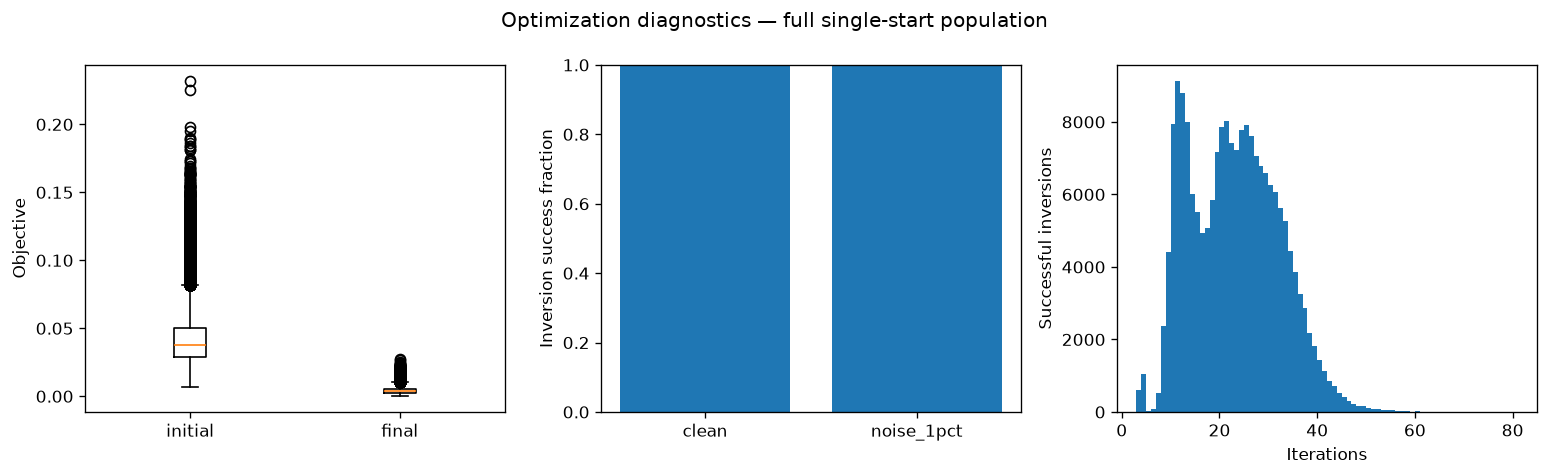
\includegraphics[width=\textwidth]{figures/optimization-diagnostics.png}
\caption{全量单起点群体优化诊断（\texttt{results/inversion-report/optimization-diagnostics.png}）：
初始/最终目标分布、两情景 100\% 成功率、迭代次数直方图。}
\label{fig:opt-diag}
\end{figure}

\textbf{频散重构（代理口径）}：恢复模型经代理预测的曲线相对观测的总体 MAE 为
0.00642 km/s（RMSE 0.0315，P95 0.0172，比较单元 95{,}760{,}266 个，无缺失）；
分模式 M0/M1/M2/M3 的 MAE 分别为 0.00284/0.00438/0.00920/0.00928 km/s。
按情景：clean 0.00503，noise\_1pct 0.00780 km/s。

\textbf{Vs 恢复（主要精度指标）}：表 \ref{tab:full-vs}。总体 Vs MAE 0.3047 km/s、
RMSE 0.4257 km/s、平均相对误差 20.82\%、P95 绝对误差 0.899 km/s。噪声的影响极小：
成对（同一样本两情景均成功）差仅 \(+5.6\times10^{-4}\) km/s（相对误差 \(+0.043\)
个百分点），说明恢复误差由结构性因素主导而非观测噪声。

\begin{table}[H]
\centering
\caption{全量单起点实验 Vs 恢复指标（按情景与模型族；行数为情景\(\times\)样本。
总体行另含 RMSE 0.4257 km/s）}
\label{tab:full-vs}
\small
\begin{tabular}{llcccc}
\toprule
情景 & 族 & 行数 & MAE (km/s) & 平均相对误差 & P95 (km/s) \\
\midrule
\multirow{4}{*}{clean}
 & normal        & 25{,}056 & 0.2694 & 17.79\% & 0.8447 \\
 & high\_velocity & 10{,}074 & 0.2639 & 17.40\% & 0.8161 \\
 & low\_velocity  & 14{,}791 & 0.3223 & 22.11\% & 0.9460 \\
 & coupled       & 50{,}079 & 0.3249 & 22.61\% & 0.9213 \\
\midrule
\multirow{4}{*}{noise\_1pct}
 & normal        & 25{,}056 & 0.2703 & 17.86\% & 0.8461 \\
 & high\_velocity & 10{,}074 & 0.2648 & 17.44\% & 0.8182 \\
 & low\_velocity  & 14{,}791 & 0.3225 & 22.12\% & 0.9473 \\
 & coupled       & 50{,}079 & 0.3253 & 22.64\% & 0.9224 \\
\midrule
\multicolumn{2}{l}{总体（两情景合并）} & 200{,}000 & 0.3047 & 20.82\% & 0.8995 \\
\bottomrule
\end{tabular}
\end{table}

正常与高速族恢复显著优于低速与耦合族（约 17\% 对 22\% 相对误差；
图 \ref{fig:vs-kind}）。误差沿深度迅速增长（图 \ref{fig:vs-depth}）：逐层 MAE 由
第 0 层的 0.003 km/s 增至 1.7 km 深度处的 0.772 km/s；偏差自约 1.1 km 起转为显著
负值（1.7 km 处 \(-0.772\) km/s），即深部速度被系统性低估。该形态与逐层搜索边界
直接相关：参考模型由基阶观测按 \(v_{\text{ph}}/(3f)\) 深度经验式构造，深部约束弱，
而 \(\pm0.35\) km/s 的边界又禁止恢复模型远离参考模型，真实模型的高速半空间
（最高 2.6 km/s）落在边界之外时即产生截断型负偏差。

\begin{figure}[H]
\centering
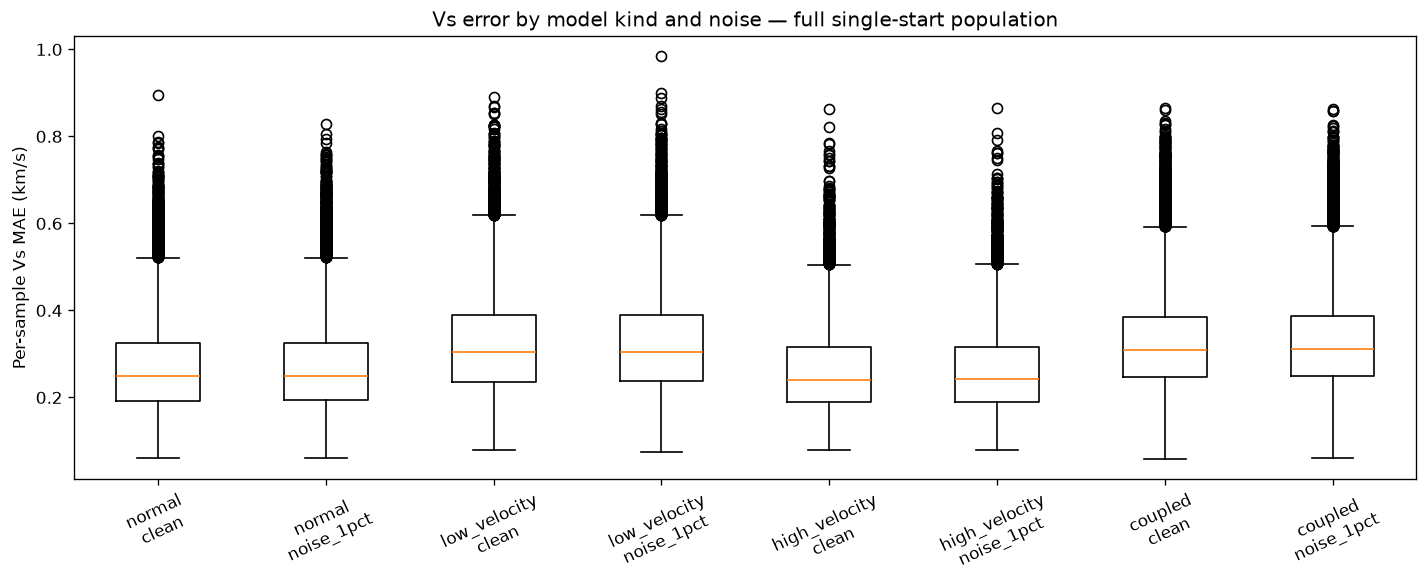
\includegraphics[width=0.95\textwidth]{figures/vs-error-by-kind-and-noise.png}
\caption{全量群体按模型族与噪声情景的单样本 Vs MAE 箱线图
（\texttt{vs-error-by-kind-and-noise.png}）。}
\label{fig:vs-kind}
\end{figure}

\begin{figure}[H]
\centering
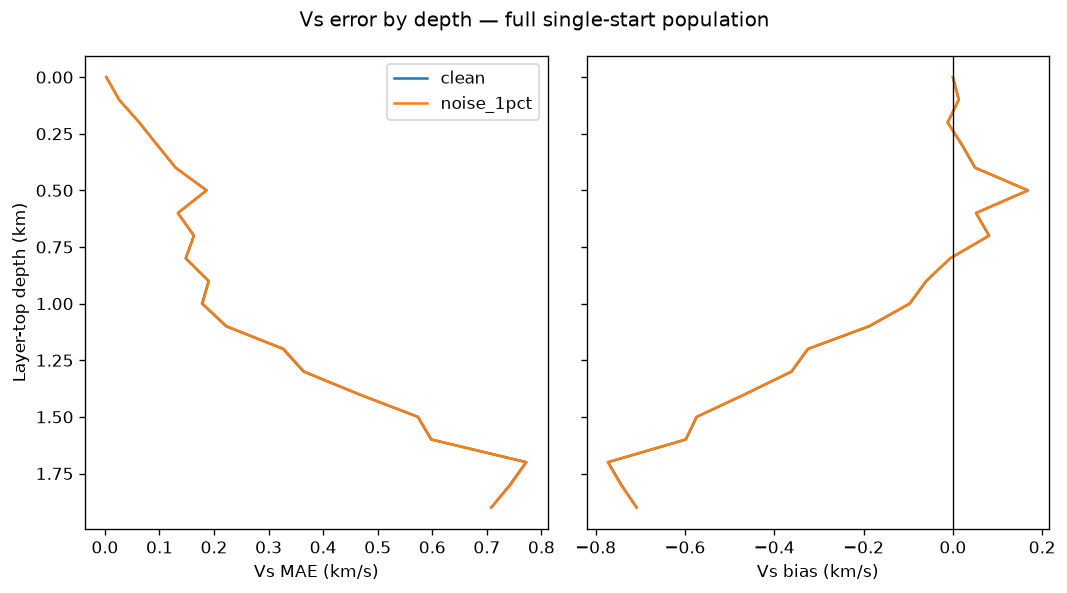
\includegraphics[width=0.95\textwidth]{figures/vs-error-by-depth.png}
\caption{全量群体逐层 Vs MAE 与偏差（\texttt{vs-error-by-depth.png}）。两情景曲线
几乎重合；深部 MAE 接近 0.8 km/s 且偏差达 \(-0.8\) km/s 量级。}
\label{fig:vs-depth}
\end{figure}

\subsection{深度多起点实验（400 样本 \(\times\) 100 起点，800 行）}
\textbf{起点诊断}：80{,}000 次起点全部收敛（100\%）；IQR 栅栏剔除 5{,}300 次
（占成功起点 6.625\%），保留内点 74{,}700 次；单样本被剔起点均值 6.6（最大 23）。
逐样本合计迭代均值 2{,}661 次（单次起点均值 26.6 次、求值 33.3 次）。
800 行全部满足``\(\geq20\) 个有效解''的成功判据。

\textbf{Vs 恢复}：总体 MAE 0.2713 km/s、RMSE 0.3906、相对误差 18.32\%、P95 0.848
（clean 0.2710，noise\_1pct 0.2715；成对差 \(+4.8\times10^{-4}\) km/s）。
分族（clean / noise\_1pct）：正常 0.2441 / 0.2458，高速 0.2418 / 0.2407，
低速 0.3128 / 0.3141，耦合 0.2855 / 0.2856 km/s。多起点相对单起点总体改善约 11\%
（0.3047 \(\to\) 0.2713 km/s），主要来自中位数集成对离群解的抑制，但量级未变。

\textbf{物理重校验}：800 行的 Dunkin 物理重算全部成功（100\%），物理频散重构
总体 MAE 0.01156 km/s（RMSE 0.0276，P95 0.0637，缺失率 0.27\%），分模式
M0--M3 为 0.0108/0.0104/0.0118/0.0132 km/s；clean 0.0102，noise\_1pct 0.0130。
值得注意的是，同一恢复模型的代理重构误差（总体 0.0155 km/s）反而\emph{大于}物理
重校验误差（0.0116 km/s）——即代理自身在该子集上的外推误差已超过物理重构误差，
代理精度成为该环节的瓶颈之一。

\textbf{不确定性区间（未达预期）}：内点起点 P10--P90 区间的总体覆盖率仅
\textbf{49.7\%}（名义 80\%），平均区间宽 0.295 km/s。逐层覆盖率从浅层的
0.95--0.98 单调退化至深部：1.2 km 以下低于 50\%，1.4--1.9 km 各层覆盖率分别为
0.049、0.021、0.003、0、0、0——深部区间完全不含真值。欠覆盖与第
\ref{sec:inversion}.1 节的系统性负偏差同源：所有起点共享同一有界搜索盒，
当真实深部速度位于盒外时，区间再宽也无法覆盖。

\subsection{代表性样本}
图 \ref{fig:rep-lvl} 与图 \ref{fig:rep-coupled} 分别展示低速族（clean）与耦合族
（noise\_1pct）的代表性深度实验样本（报告器选取规则：各族成功深样本中的最小
样本 ID）。两图共同呈现了本研究的核心现象：
右四幅子图中恢复模型的代理与物理频散曲线与观测几乎重合，而左幅 Vs 剖面中，
中位数恢复模型明显更平滑、深部幅度远低于真值，P10--P90 带在深部亦未能包住真值。
频散拟合优度不能作为 Vs 恢复质量的充分判据。

\begin{figure}[H]
\centering
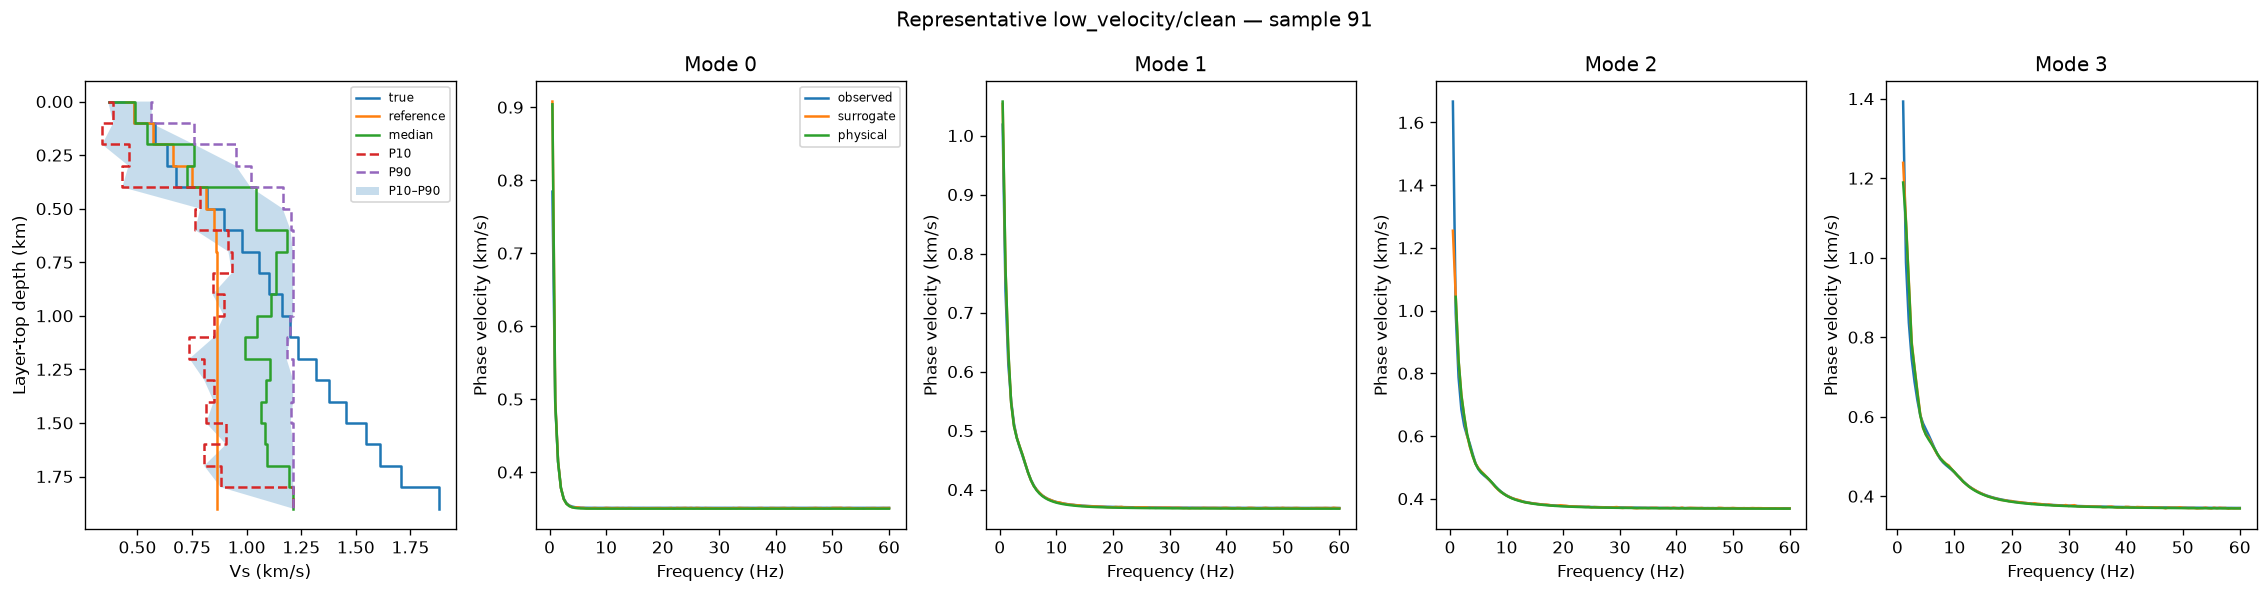
\includegraphics[width=\textwidth]{figures/representative-low_velocity-clean.png}
\caption{代表性低速族样本（clean，样本 91；\texttt{representative-low\_velocity-clean.png}）。
左：真值/参考/中位数/P10/P90 Vs 剖面；右四幅：M0--M3 观测、代理与物理重构曲线。}
\label{fig:rep-lvl}
\end{figure}

\begin{figure}[H]
\centering
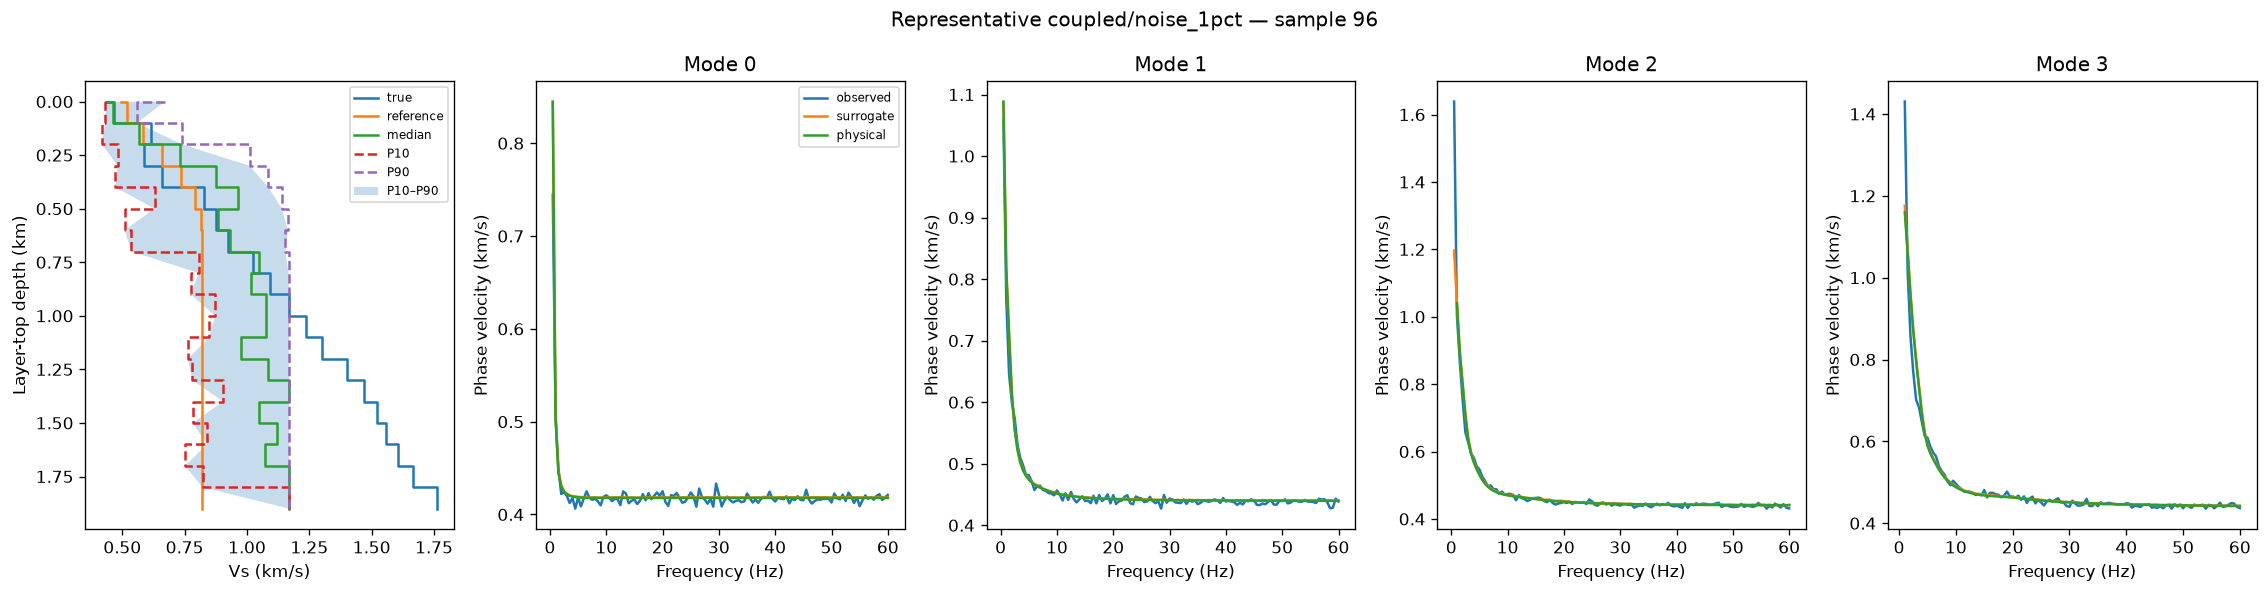
\includegraphics[width=\textwidth]{figures/representative-coupled-noise_1pct.png}
\caption{代表性耦合族样本（noise\_1pct，样本 96；
\texttt{representative-coupled-noise\_1pct.png}）。1\% 噪声下频散重构仍近乎重合，
但深部 Vs 恢复显著失真。}
\label{fig:rep-coupled}
\end{figure}

\section{监督反演基线与外部参考}\label{sec:invnet}
InverseNet（第 \ref{sec:inv-method}.6 节口径，独立分折）训练 3 个种子，各 150 轮内
早停于验证 MSE 最优。日志记录：种子 0 最佳验证 MAE 26.74 m/s、测试 MAE
\textbf{26.87 m/s}；种子 1 验证 26.58 m/s；种子 2 验证 26.54 m/s；两种子集成测试
MAE \textbf{26.08 m/s}（\((50{,}000\times20)\) 预测已保存但当时日志未记录三种子
集成数值）。对比优化反演（全量 304.7 m/s、深度 271.3 m/s MAE），监督基线低约一个
数量级。

外部参考（iNETT 姊妹项目归档，单位以其文件记录为准，测试折 \(\geq95\)）：
iCNN 总体 MAE 0.0746 km/s、RMSE 0.1115、\(R^2=0.749\)（\(n=50{,}000\)）；
iNETT 总体 MAE 0.0635 km/s、RMSE 0.1051、\(R^2=0.795\)（\(n=2{,}000\) 子集）；
linear 基线发散（MAE 5.04、\(R^2=-1874\)），其逐层误差在深部达两位数 km/s，
不具备物理意义。图 \ref{fig:inett} 为其归档的逐样本剖面对比。

\begin{figure}[H]
\centering
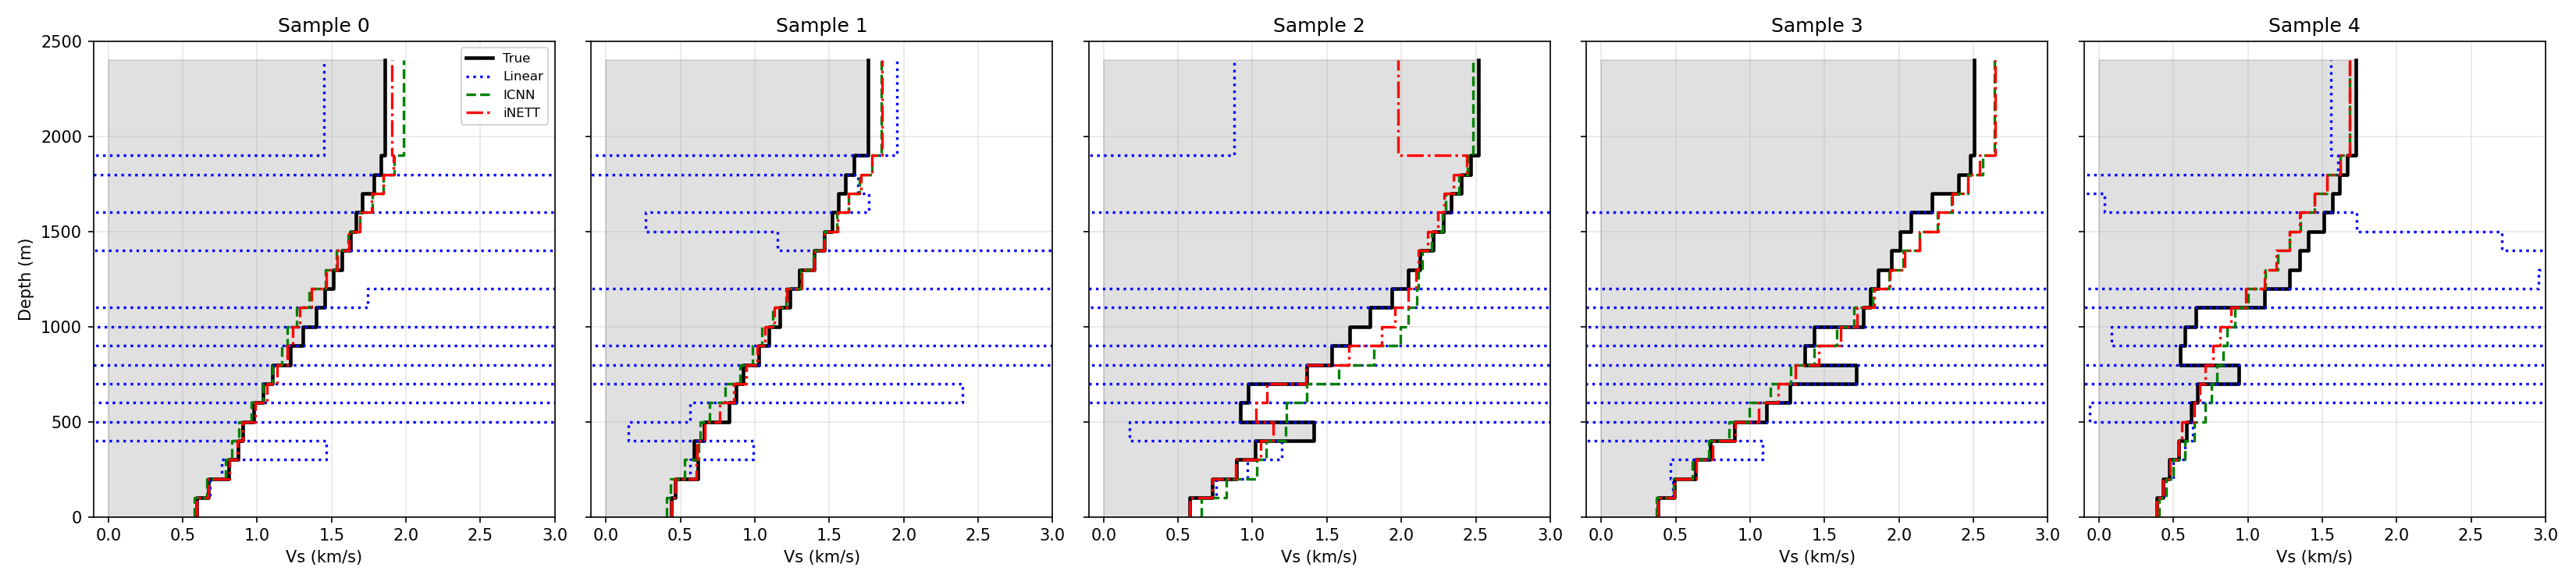
\includegraphics[width=\textwidth]{figures/inett-vs-comparison-all.png}
\caption{iNETT 姊妹项目归档的 5 个测试样本剖面对比（来源：
\texttt{iNETT-.../results/swave\_inversion/vs\_comparison\_all.png}）。linear 基线
发散；iCNN 与 iNETT 能跟踪真值剖面总体形态。}
\label{fig:inett}
\end{figure}

\textbf{可比性警示}：InverseNet 与 iCNN/iNETT 的训练折（\(<90\)）覆盖了主管线
\texttt{mod100-v2} 的反演保留行（90--99），故其测试指标对主管线协议而言含训练泄漏，
不能据此断言监督方法在同等协议下仍领先一个数量级；该差距应理解为\emph{协议不对称
的参考值}，并在第 \ref{sec:discussion} 节讨论其合理成因与后续验证方案。

另需如实说明：混合反演流程（InverseNet 初值 + 可微代理上的批量投影 Adam 精修，
\texttt{run\_hybrid}）的源码仅存字节码，其运行输出（对比指标、预测文件）未在仓库
或姊妹项目结果目录中找到——该实验线\emph{未留下可归档的结果}，本报告不包含其结论。

\section{讨论}\label{sec:discussion}

\paragraph{拟合--恢复分离：非唯一性是主要误差源}
反演在所有 20.08 万行上 100\% 收敛且频散重构 MAE 达 \(10^{-3}\) km/s 量级，
但 Vs MAE 高达 0.27--0.30 km/s。这说明目标函数的极小值域包含大量与真值差异巨大
的等效模型：观测（4 模式 \(\times\) 120 频点）不足以在 20 维模型空间内唯一确定
深部结构。1\% 噪声几乎不改变恢复精度（成对差 \(+5\times10^{-4}\) km/s）进一步证实
误差预算由结构性非唯一性与先验约束主导，而非数据质量。

\paragraph{边界约束的系统性偏差}
逐层边界取自基阶经验深度式构造的参考模型（\(\pm0.35\) km/s）。浅部该近似有效
（第 0 层 MAE 仅 0.003 km/s），但深部灵敏度低、经验深度式失真，真实半空间速度常
落于界外，造成 1.1 km 以下单调增长的负偏差（最大 \(-0.772\) km/s）与区间零覆盖。
这是本管线当前最明确的可改进点：放宽深部边界、引入多参考模型或对边界本身做
分层标定，都可能显著降低深部误差。

\paragraph{不确定性量化不可用}
P10--P90 经验区间总体覆盖率 49.7\%（名义 80\%）且深部为零，表明``同一搜索盒内
多起点的散布''不能刻画真实后验不确定性。任何下游应用不应直接使用该区间。

\paragraph{代理精度的双重角色}
深度子集上代理重构误差（0.0155 km/s）大于物理重校验误差（0.0116 km/s），说明
在恢复模型分布上代理外推误差已超过物理拟合残差。当前划分检查点缺少归档的独立
测试集评估（第 \ref{sec:surrogate} 节），是证据链上的一个缺口；虽然旧划分检查点的
测试指标（表 \ref{tab:oldsplit-eval}）与全量实验的频散重构量级相互印证，正式结论
仍应以待补做的评估为准。

\paragraph{监督基线的领先及其解释}
InverseNet（约 27 m/s MAE）较优化反演（约 300 m/s）低一个数量级。即便剔除协议
不对称因素，这一差距有合理成因：优化反演的目标只含数据拟合与弱光滑先验，在
非唯一方向上自由滑动；监督网络学习的是条件均值 \(E[V_s\mid d]\)，隐式利用了训练
分布的先验（包括深部高速半空间的统计形态），恰好补上优化目标缺失的约束。这提示
两条技术路线的结合——以监督初值约束优化搜索（混合法）——是最有前景的方向；
但当前混合法实验未留下可归档结果，该结论尚待验证。严格的可比结论需要在
\texttt{mod100-v2} 协议下重训监督基线（训练折剔除 90--99 行）后再做对比。

\paragraph{工程完整性}
结果模式 v3 将数据集清单、检查点、配置、源码摘要与精确样本身份绑定；分片原子发布、
断点恢复与任务模划分均经损坏/恢复类测试验证。全部 226 项单元与集成测试通过
（约 99 s），\texttt{ruff} 检查零告警（2026-08-10 本机复核）。

\section{结论}\label{sec:conclusion}
本项目交付了从确定性数据生成、物理正演、神经代理到可审计反演实验的完整管线，
并完成了百万样本数据集、300 轮代理训练、20 万行全量反演与 8 万起点的深度多起点
实验。结果喜忧参半，且均有据可查：正演与代理环节精度优异（验证 MAE
\(1.82\times10^{-4}\) km/s）；反演环节则暴露了非唯一性主导的本质困难——
完美的频散拟合并未转化为可用的 Vs 恢复（MAE 0.27--0.30 km/s），经验不确定性区间
严重欠覆盖（49.7\%），深部存在边界约束导致的系统性负偏差。监督直接反演基线以
低约一个数量级的误差（26.9 m/s，协议不对称，仅供参考）指明了引入学习型先验的
必要性。后续工作的优先级：（1）补做当前检查点的独立测试集正演评估；
（2）重新设计深部边界/参考模型；（3）在 \texttt{mod100-v2} 协议下重训监督基线并
完成混合反演实验；（4）用物理重校验替代代理口径作为反演成功判据的可选路径。

\appendix
\section{可复现性与产物清单}\label{app:repro}
\begin{sloppypar}
\begin{itemize}
\item 代码：\texttt{src/swave/} 20 个模块约 7{,}946 行；测试 21 个文件；
      仓库 39 次提交（\texttt{main}，最新 \texttt{591cda0}）。
\item 测试：\texttt{python -m pytest -q} \(\to\) 226 passed（98.84 s）；
      \texttt{ruff check src tests scripts} \(\to\) All checks passed（2026-08-10）。
\item 数据：\texttt{data/production}（100 分片，清单逐片 SHA-256，完整完成）；
      基准副本 \texttt{data/production-w64}（同种子，分片哈希不同）。
\item 检查点：\texttt{runs/production-48g/\{best,last\}.pt}（当前划分，反演兼容）；
      \texttt{runs/production-48g-old-split/}（旧划分，含测试评估，协议隔离）。
\item 反演结果：\texttt{results/inversion}（282 个结果/锁文件，原子发布）；
      报告 \texttt{results/inversion-report/\{summary.json + 11 幅图\}}。
\item 关键身份绑定（结果模式 v3）：数据集清单 SHA-256
      \texttt{ceecda31ae9dec3f\ldots}；检查点 \texttt{b1a6fc08a40ba648\ldots}；
      源码摘要 \texttt{06f66599106b57f2\ldots}；划分 \texttt{mod100-v2-80-5-5-10}。
\item 复算命令：\texttt{python -m pytest -q}；
      \texttt{swave inversion-report --results-dir results/inversion
      --dataset-dir data/production --output-dir results/inversion-report}。
\item 已知缺口：当前检查点独立测试集评估未归档；生产训练/生成的主机与耗时未归档
      （外部机器执行）；\texttt{logs/production-pipeline.log} 仅存一行失败记录；
      InverseNet/混合法源码仅存字节码，混合法结果未归档。
\end{itemize}
\end{sloppypar}

\end{document}
